% !TEX root = TD_fluides_part1.tex

\setcounter{section}{2}
\section{Cinématique}

\setcounter{subsection}{-1}

%%%%%%%%%%%%%%%%%%%%%%%%%%%%%%%%%%%%%%%%%%%%%%%%%%%%%%%%%%%%%%%%%
\subsection{\'Ecoulement de d\'eformation pure (exercice corrigé sur moodle)}
%%%%%%%%%%%%%%%%%%%%%%%%%%%%%%%%%%%%%%%%%%%%%%%%%%%%%%%%%%%%%%%%%


On consid\`ere l'\'ecoulement plan
d\'efini par le champ de vitesse : 
\begin{equation*}
\left\{
\begin{array}{ccr}
u(x,y) & = & a x +b y \\ 
v(x,y) & = & cx + dy
\end{array}
\right.
\text{o\`u $a$,$b$,$c$  et $d$ sont des constantes.}
\end{equation*}
\begin{enumerate}


\item Donnez l'expression du tenseur des taux de déformation, de la divergence puis de la vorticité correspondant à cet écoulement.

\item Que vaut l'accélération ? celle-ci est-elle uniforme ?

\item Dans le cas $d=-a$, justifiez qu'on peut introduire une fonction de courant $\psi(x,y)$ pour décrire l'écoulement, et donnez son expression.

\item Déterminez les lignes de courant et les trajectoires (on vérifiera qu'il s'agit des mêmes courbes).

\item A l'aide du programme Matlab disponible sur moodle, tracez la structure de l'écoulement dans les cas suivants :
\begin{description}
\item{$(i)$} $b=1$, $a=c=d=0$.
\item{$(i)$} $a=1$, $b=c=0$, $d=-1$.
\item{$(i)$} $b=c=1$, $a=d=0$.
\end{description}

\item Justifiez pourquoi ces deux derniers cas définissent le même écoulement.

\end{enumerate}
%\clearpage




%%%%%%%%%%%%%%%%%%%%%%%%%%%%%%%%%%%%%%%%%%%%%%%%%%%%%%%%%%%%%%%%%
\subsection{Tourbillon de vidange}
%%%%%%%%%%%%%%%%%%%%%%%%%%%%%%%%%%%%%%%%%%%%%%%%%%%%%%%%%%%%%%%%%


On étudie un écoulement stationnaire,
occupant un récipient cylindrique de rayon $R_0$ et de hauteur $H$.
 
Le champ de vitesse est donné en coordonnées cylindriques
par $\vec u = u_r \vec e_r + u_\theta \vec e_\theta  + u_z \vec e_z$,
avec les expressions suivantes :

$$
\mbox{ pour } r<a : \quad 
\left\{ 
\begin{array}{lcr}
u_r &=& \displaystyle - \frac{Dr}{2 \pi a^2}\\ \\
u_\theta &=& \displaystyle \frac{\Gamma r }{2 \pi a^2}\\ \\
u_z&=& \displaystyle \frac{D z}{\pi a^2}  
\end{array}
\right. 
\qquad  \qquad
\mbox{ pour } r>a :
\quad
\left\{ 
\begin{array}{lcr}
u_r &=& - \displaystyle \frac{D}{2 \pi r}\\ 
\\
u_\theta &=& \displaystyle \frac{\Gamma}{2 \pi r}\\
\\
u_z&=& 0  
\end{array}
\right. 
$$
 
\paragraph{Partie A :  "Tourbillon de Rankine" }  $ \, $

On considère tout d'abord l'écoulement plan correspondant à $D = 0$ , $\Gamma > 0$.



\begin{enumerate}

\item Donnez l'expression du tenseur des gradients de vitesse dans chacune des deux régions de l'écoulement. En déduire la divergence, la vorticité $\vec \omega$ puis le tenseur des taux de déformations $\tensor{D}$.

\item 
Représentez schématiquement les déformations d'un volume élémentaire $dV = r d\theta dr dz$ situé dans le coeur ($r<a$) puis dans la zone extérieure ($r>a$).

\item Après avoir justifié son existence, donnez l'expression de la fonction de courant $\psi$ associée à cet écoulement. En déduire que les lignes de courant sont des cercles concentriques.

\item (question facultative) Reprendre l'étude à partir d'une description en coordonnées cartésiennes $u_x(x,y) \vec e_x  + u_y(x,y)  \vec e_y $. 

\paragraph{Partie B :  "Ecoulement de vidange non tournant" }  $ \, $

On considère maintenant l'écoulement à symétrie de révolution correspondant à $D > 0$ , $\Gamma = 0$.


\item Donnez l'expression du tenseur des gradients de vitesse. En déduire la divergence, la vorticité $\vec \omega$ puis le tenseur des taux de déformations $\vec{D}$.

\item 
Représentez schématiquement les déformations d'un volume élémentaire $dV = r d\theta dr dz$ situé dans la zone extérieure ($r>a$) puis dans le coeur $r<a$).

\item Après avoir justifié son existence, donnez l'expression de la fonction de Stokes $\Psi$ associée à cet écoulement. En déduire la géométrie des lignes de courant.

\item Calculez le flux volumique A travers la paroi latérale du cylindre ($r=R_0$) puis à travers le fond du récipient ($z=H$).


\paragraph{Partie C :  "Tourbillon de vidange" }  $ \, $

%\vspace{.1cm}

On considère maintenant le cas général : $D > 0$ , $\Gamma > 0$.

\item Calculez la {\em trajectoire} (paramétrée sous la forme $[R(t) ; \theta(t) ; Z(t)]$ ) 
d'une particule fluide située initialement à la position $[R(0) = R_0, \theta(0) = \theta_0, Z(0) = Z_0]$.
Montrez que celle-ci est donnée par :

$$
\small
 \mbox{ pour } t<t_c : \quad
\left\{ 
\begin{array}{lcl}
R(t) &=& \sqrt{R_0^2 - \frac{D t}{2 \pi} }
 \\ \\
\theta(t) &=& \displaystyle \theta_0 - \frac{\Gamma}{D}  \frac{ ln \left( R_0^2 - D t/(2 \pi) \right)}
{  ln (R_0^2) };   \\
\\
Z(t) &=& Z_0 
\end{array}
\right. 
\quad
\mbox{ pour } t>t_c :
\left\{ 
\begin{array}{lcl}
R(t) &=& \displaystyle a \exp \left( - \frac{D (t-t_c)}{2 \pi} \right) \\ \\
\theta(t) &=& \displaystyle \theta_c + \frac{\Gamma}{2 \pi} (t-t_c)  \\
\\
Z(t) &=& \displaystyle Z_0 + Z_0  \exp \left( \frac{D (t-t_c)}{ \pi} \right) 
\end{array}
\right. 
$$ 



Avec  : 
$$
t_c  = \frac{2\pi  (R_0^2- a^2)}{D} ; \quad \quad 
\theta_c = \theta_0 - \frac{\Gamma}{D}  \frac{ ln (a^2  ) }{  ln (R_0^2) }   .
$$


\item Vérifiez que les projections dans un plan horizontal des trajectoires sont des spirales d'Archimède d'équation $r \equiv e^{-\alpha \theta}$ et donnez le "pas" de la spirale $\alpha$ en fonction de $\Gamma$ et $D$. 

\item Retrouvez ce résultat plus simplement en étudiant les {\em lignes de courant} de l'écoulement.

\item Représentez schématiquement la forme des trajectoires (ou des lignes de courant) de l'écoulement tridimensionnel.

\end{enumerate}



 





%%%%%%%%%%%%%%%%%%%%%%%%%%%%%%%%%%%%%%%%%%%%%%%%%%%%%%%%%%%%%%%%%
\subsection{\'Ecoulement instationnaire}
%%%%%%%%%%%%%%%%%%%%%%%%%%%%%%%%%%%%%%%%%%%%%%%%%%%%%%%%%%%%%%%%%


On consid\`ere un \'ecoulement bidimensionnel dont la vitesse 
est donn\'ee sous forme eulérienne par :
\begin{equation*}
\left\{
\begin{array}{rcc}
u_x(x,y,t) & = & U_0 \cos \omega t, \\
u_y(x,y,t) & = & U_0 \sin \omega t. 
\end{array}
\right.
\end{equation*}

\begin{enumerate}

\item Donnez la forme des lignes de courant en un instant $t$ donné.
Représentez le champ de vitesse pour 4 instants correspondant 
à $t=0$, $t=T/4$, $t=T/2$, et $t=3T/4$, où 
$T = 2 \pi / \omega$ est la période du cycle.


\item On note $\vec X(t; \vec x_0, t_0)$ la position lagrangienne, à l'instant
$t$, de la particule fluide qui était située à la position $\vec x_0$  
à l'instant $t_0$. 

Calculez les composantes de $\vec X(t; \vec x_0, t_0)$,
notées  $X(t; x_0,y_0,t_0)$ et  $Y(t; x_0,y_0,t_0)$,
où $x_0$ et $y_0$ sont les composantes de $\vec x_0$.


\item Quelle est la forme des trajectoires ? Représentez la trajectoire
de 4 particules, correspondant respectivement à
$(x_0,y_0,t_0) = (0,0,0)$ ;  $(0,0,T/4)$ ; $(0,0,T/2)$ ; et $(0,0,3T/4)$.


\item Quelle est la forme des lignes d'émission ?
Représentez la ligne d'émission correspondant au 
point d'émission $\vec x_0 = \vec 0$, en quatre instants, 
correspondant à $t=0$, $t=T/4$, $t=T/2$, et $t=3T/4$. 

\end{enumerate}



%%%%%%%%%%%%%%%%%%%%%%%%%%%%%%%%%%%%%%%%%%%%%%%%%%%%%%%%%%%%%%%%%
\subsection{\'Ecoulement stationnaire accéléré dans une conduite}
%%%%%%%%%%%%%%%%%%%%%%%%%%%%%%%%%%%%%%%%%%%%%%%%%%%%%%%%%%%%%%%%%


On étudie l'écoulement dans une conduite rectiligne de 
section constante $S$. L'écoulement est monodirectionnel et stationnaire,
et on pose  $\vec u (\vec x, t) =  U(x)\vec e_x$.
L'écoulement subit une accélération dans la portion de conduite située
entre $x=0$ et $x=L$. 
De part et d'autre de cette zone l'écoulement est uniforme.
De manière plus précise, on suppose que le champ de vitesse est 
donné par la définition (eulérienne) suivante :

$$
U(x) = \left\{ 
\begin{array}{ll} 
U_0 &  \mbox{ pour } x<0; \\
U_0+ \alpha x & \mbox{ pour }  0<x<L; \\
U_1 &\mbox{ pour } x>L,  \mbox{ avec }  U_1 = U_0 + \alpha L. \\
\end{array}
\right.
$$

Cet écoulement modélise (très simplement) l'écoulement dans un
turboréacteur.

\begin{enumerate}

\item Calculez la divergence du champ de vitesse.

\item On note $X(t)$ la position lagrangienne de la particule
fluide située à l'origine du repère à $t_0 = 0$. Calculez $X(t)$.

\item Calculez la vitesse lagrangienne $U(t)$ et l'accélération 
lagrangienne $A(t)$ de cette particule fluide.

\item Exprimez l'accélération en variables euleriennes.  
Montrez qu'on a bien $A = \partial U / \partial t + U \partial U / \partial x$.

\item Donnez l'expression du débit massique à travers la conduite.
En écrivant que ce dernier est constant, en déduire la loi eulerienne
de masse volumique, $\rho(x)$.

\item Donnez la loi lagrangienne de masse volumique, $ \rho(t)$, de
la particule fluide considérée prédédemment.

\item Calculez la dérivée particulaire de la masse volumique, $d\rho/dt$.
Vérifiez que l'on a bien $d\rho / dt + \rho div (\vec u) = 0$.

  
\end{enumerate}



\comment{
%%%%%%%%%%%%%%%%%%%%%%%%%%%%%%%%%%%%%%%%%%%%%%%%%%%%%%%%%%%%%%%%%
\subsection{\'Ecoulement de d\'eformation pure}
%%%%%%%%%%%%%%%%%%%%%%%%%%%%%%%%%%%%%%%%%%%%%%%%%%%%%%%%%%%%%%%%%


On consid\`ere l'\'ecoulement plan
d\'efini par le champ de vitesse : 
\begin{equation*}
\left\{
\begin{array}{ccr}
u(x,y) & = & a x \\ 
v(x,y) & = & - a y
\end{array}
\right.
\text{o\`u $a$ est une constante.}
\end{equation*}
\begin{enumerate}
\item V\'erifier que l'\'ecoulement est incompressible, irrotationnel
et stationnaire.
\item D\'eterminer l'expression de la fonction de courant $\psi(x,y)$.
\item Ecrire l'\'equation des lignes de courant.  Indiquer la nature
  de ces courbes.
\item Calculer la trajectoire d'un point plac\'e initialement en $(X_0, Y_0)$.
\item Un ensemble de particules fluides plac\'ees initialement le long
d'un segment horizontal restent-elles dispos\'ees le long d'un segment
horizontal tout au long de leur \'evolution ? En est-il de m\^eme si elles
sont plac\'ees initialement sur un segment vertical ?
\item En d\'eduire l'\'evolution du volume fluide repr\'esent\'e sur la
figure suivante. Quelle transformation subit-il au cours de son mouvement ?
\begin{figure}[htb]
  \centering
  \setlength{\unitlength}{1cm}
  \begin{picture}(10,7.5)
    \put(0,0){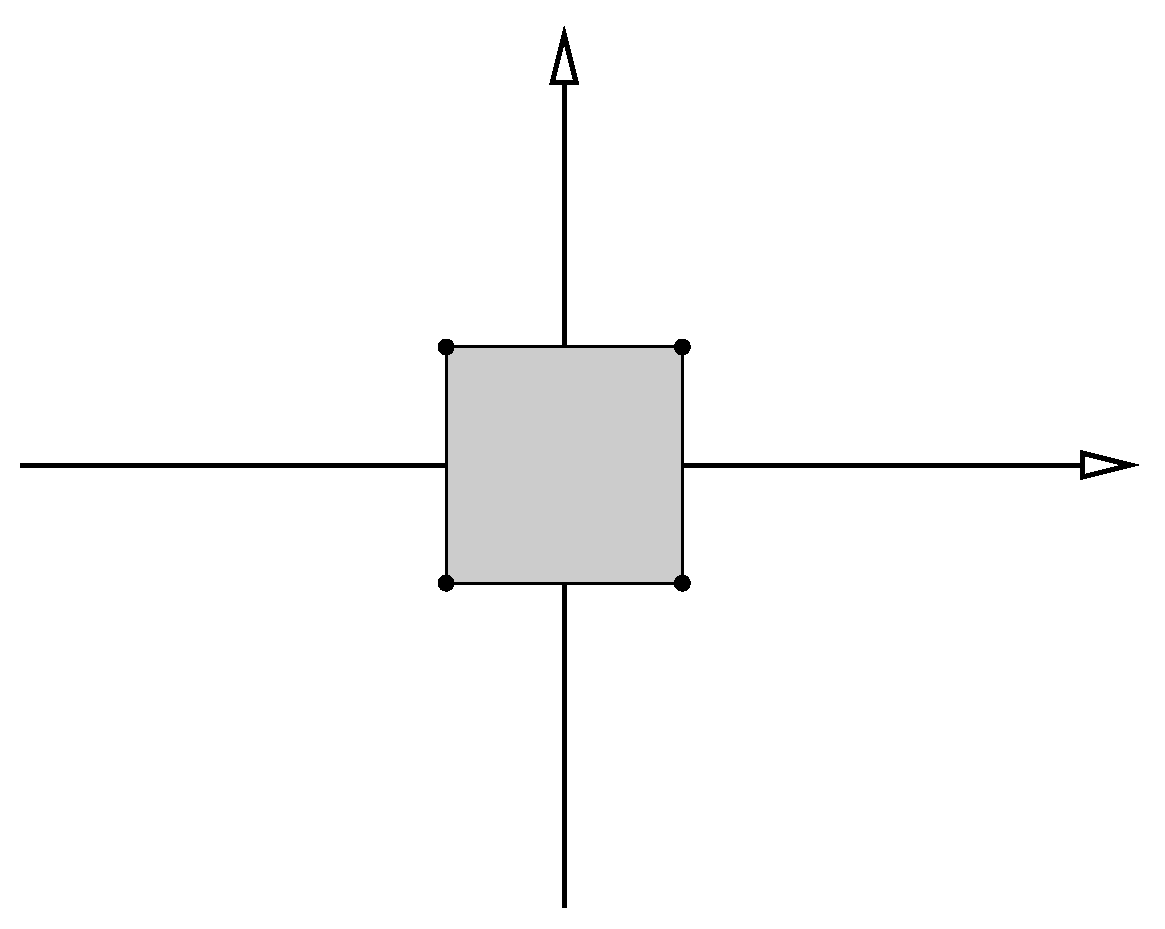
\includegraphics[width=10cm]{./deformation.eps}}
    \put(9.5,3.3){$x$}
    \put(4.3,7.5){$y$}
    \put(3.7,5.6){$A$}
    \put(5.8,5.6){$B$}
    \put(3.2,5.2){$(-1,1)$}
    \put(5.5,5.2){$(1,1)$}
    \put(3.6,2.4){$D$}
    \put(5.7,2.4){$C$}
    \put(2.9,2){$(-1,-1)$}
    \put(5.2,2){$(1,-1)$}
  \end{picture}
  \caption{\'El\'ement de volume \`a l'instant initial.}
  \label{fig:deformation}
\end{figure}
\item Comment pourrait-on g\'en\'erer ce type d'\'ecoulement ? Citer des
exemples d'\'ecoulements r\'eels pr\'esentant ces caract\'eristiques.
\end{enumerate}
}


%%%%%%%%%%%%%%%%%%%%%%%%%%%%%%%%%%%%%%%%%%%%%%%%%%%%%%%%%%%%%%%%%%%%%%
\subsection{Descriptions lagrangienne et eul\'erienne 
{\small \it (Partiel 2004)}}
%%%%%%%%%%%%%%%%%%%%%%%%%%%%%%%%%%%%%%%%%%%%%%%%%%%%%%%%%%%%%%%%%%%%%%


On consid\`ere l'\'ecoulement suivant donn\'e sous forme 
\textit{lagrangienne} :
\begin{equation*}
\left\{
\begin{array}{rcl}
X(t) & = & b t + X_0 \\
Y(t) & = & \frac{a}{\omega} \sin(\omega t) + Y_0
\end{array}
\right.
\text{o\`u $a$, $b$ et $\omega$ sont des constantes.}
\end{equation*}
\begin{enumerate}
\item Donner l'\'equation des trajectoires $Y(X)$.
\item Donner la signification physique de $X_0$ et $Y_0$.
\item Calculer l'acc\'el\'eration lagrangienne $\vec{a}_L$.
\item Donner la description eul\'erienne de ce mouvement.
Calculer le terme convectif. En d\'eduire l'acc\'el\'eration
eul\'erienne $\vec{a}_E$. Comparer avec $\vec{a}_L$.
\item Ce mouvement est-il stationnaire ? isovolume ? irrotationnel ?
\item D\'eterminer l'\'equation des lignes de courant. On en pr\'ecisera
la forme g\'eom\'etrique.
\item Tracer les trajectoires correspondant aux trois conditions initiales :
$X_0 = 0$ et $Y_0 = -1, 0$ et $1$.
\item Tracer sur le m\^eme graphe les lignes de courant pour $y_0 = -1, 0$
et $1$ aux instants $t = 0, 0.5$ et $1$ seconde. On prendra 
$b = 1$ m.s$^{-1}$, $a = 2 \pi$ m.s$^{-1}$ et $\omega = 2 \pi$ rad.s$^{-1}$.
\end{enumerate}



%%%%%%%%%%%%%%%%%%%%%%%%%%%%%%%%%%%%%%%%%%%%%%%%%%%%%%%%%%%%%%%%%%%%%%%%%%%
\subsection{\'Ecoulement instationnaire}
%%%%%%%%%%%%%%%%%%%%%%%%%%%%%%%%%%%%%%%%%%%%%%%%%%%%%%%%%%%%%%%%%%%%%%%%%%%


On consid\`ere l'\'ecoulement plan \textit{instationnaire} d\'efini
par $u = 1$ et $v = t$.
\begin{enumerate}
\item V\'erifier que l'\'ecoulement est incompressible.
\item D\'eterminer :
  \begin{itemize}
  \item[$\bullet$] les lignes de courant,
  \item[$\bullet$] les trajectoires,
  \item[$\bullet$] les lignes d'\'emission.
  \end{itemize}
\end{enumerate}



